\chapter[Introdução]{Introdução}
\label{cap:introducao}

\section{Importância do Trabalho e Contextualização}

\subsection{Por que este trabalho é importante?}

A dengue representa um dos desafios de saúde pública global da atualidade, especialmente em regiões tropicais e subtropicais. A Organização Mundial da Saúde (OMS) estima que aproximadamente 3,9 bilhões de pessoas — equivalente a metade da população mundial — vivem em áreas com risco de infecção por dengue. A incidência global da doença aumentou vertiginosamente nas últimas quatro décadas, passando de cerca de meio milhão de casos notificados em 2000 para 5,2 milhões em 2019, representando um crescimento superior a 1000\% \cite{naish2014climate}.

No Brasil, o cenário epidemiológico caracteriza-se por uma hiperendemicidade, com a co-circulação simultânea dos quatro sorotipos virais (DENV-1, DENV-2, DENV-3 e DENV-4). O país enfrenta epidemias cíclicas e sazonais que impõem uma carga severa e recorrente ao Sistema Único de Saúde (SUS) \cite{mussumeci2020large, roster2022machine}. Dados oficiais do Ministério da Saúde revelam que, apenas no primeiro semestre de 2024, foram notificados 6 milhões de casos prováveis de dengue em todo o território nacional, superando os registros históricos anteriores e evidenciando a dimensão continental do problema sanitário \cite{sinan2025}.

O Distrito Federal (DF), ponto de partida desta pesquisa, apresenta características epidemiológicas e climáticas relevantes para análise da dinâmica de transmissão da dengue. Localizado no bioma Cerrado, o DF apresenta características climáticas específicas que modulam sazonalmente a dinâmica de transmissão: um regime pluviométrico bem definido, alternando entre uma estação seca (aproximadamente de maio a setembro) e uma chuvosa (outubro a abril), criando condições cíclicas para a proliferação do vetor \textit{Aedes aegypti}.

O levantamento realizado na primeira etapa deste trabalho (TCC~1), a partir das bases do Sistema de Informação de Agravos de Notificação (SINAN) e do Instituto Nacional de Meteorologia (INMET) \cite{sinan2025, inmet2025}, mostrou que o ano de 2024 caracterizou-se por uma epidemia sem precedentes históricos recentes no Distrito Federal, totalizando \textbf{313.317 casos} notificados. Este volume representa um aumento de 360\% em relação ao ano anterior (64.897 casos em 2023) e supera a soma de toda a série histórica recente dos anos anteriores. A média semanal de casos passou de aproximadamente 1.247 casos por semana em 2022 para 5.927 casos por semana em 2024, evidenciando uma mudança de escala epidemiológica.

O pico dessa crise ocorreu na semana epidemiológica iniciada em 18 de fevereiro de 2024, quando o sistema de saúde registrou \textbf{25.714 casos em apenas sete dias} — uma magnitude que evidencia a incapacidade dos métodos tradicionais de vigilância epidemiológica em antecipar eventos extremos, e também o colapso subsequente dos serviços de saúde. Relatos da mídia e documentos oficiais da Secretaria de Saúde do DF descreveram unidades hospitalares operando além da capacidade, com pacientes aguardando atendimento em corredores, esgotamento de insumos básicos (soro fisiológico, medicamentos para controle de dor e febre), e comprometimento do atendimento a outras patologias urgentes, incluindo emergências cardíacas e neurológicas.

Este trabalho é importante porque busca transicionar o paradigma da vigilância epidemiológica de uma abordagem \textbf{reativa} ("o que aconteceu?") para uma abordagem \textbf{preditiva e proativa} ("o que vai acontecer e quando?"). Os métodos tradicionais de vigilância operam com base em notificações clínicas e laboratoriais, que são naturalmente defasadas em relação ao momento real da transmissão viral na comunidade. Existe um intervalo crítico de várias semanas entre a ocorrência de um evento ambiental (ex: chuva intensa) e a manifestação clínica dos primeiros casos, período durante o qual a transmissão já está ocorrendo silenciosamente.

\subsection{Do que se trata o assunto abordado?}

A dengue é uma arbovirose sistêmica de evolução benigna na maioria dos casos (aproximadamente 70-80\%), mas que pode apresentar manifestações graves e potencialmente letais. O agente etiológico é um vírus de RNA de fita simples e polaridade positiva (DENV), pertencente à família \textit{Flaviviridae} e ao gênero \textit{Flavivirus}, que compartilha características filogenéticas com outros vírus de importância médica, como os causadores da febre amarela, Zika e chikungunya.

O vírus da dengue possui quatro sorotipos antigenicamente distintos e geneticamente relacionados (DENV-1, DENV-2, DENV-3 e DENV-4), cada um com características epidemiológicas e patogênicas próprias. Estudos moleculares revelam que esses sorotipos divergiram de um ancestral comum há aproximadamente 1.000 anos, e sua diferenciação continua através de mutações acumuladas ao longo do tempo, gerando diferentes genótipos e linhagens dentro de cada sorotipo.

A transmissão ocorre primariamente pela picada de fêmeas infectadas de mosquitos do gênero \textit{Aedes}, sendo o \textit{Aedes aegypti} o vetor primário em áreas urbanas e o \textit{Aedes albopictus} um vetor secundário com potencial crescente de adaptação a ambientes periurbanos e rurais. O \textit{Aedes aegypti} é uma espécie altamente antropofílica, demonstrando preferência marcada por se alimentar de sangue humano, o que aumenta sua eficiência como vetor em áreas urbanas densamente povoadas. O mosquito se infecta ao picar um indivíduo virêmico (portador do vírus na corrente sanguínea) e, após um período de incubação extrínseco (PIE) que varia de 8 a 12 dias dependendo da temperatura ambiente, torna-se capaz de transmitir o vírus a novos hospedeiros humanos durante múltiplos repastos sanguíneos ao longo de sua vida adulta, que pode durar de 2 a 4 semanas em condições ideais.


\begin{figure}[htb]
	\centering
	\caption{\textit{Aedes aegypti}, principal vetor da dengue em áreas urbanas}
	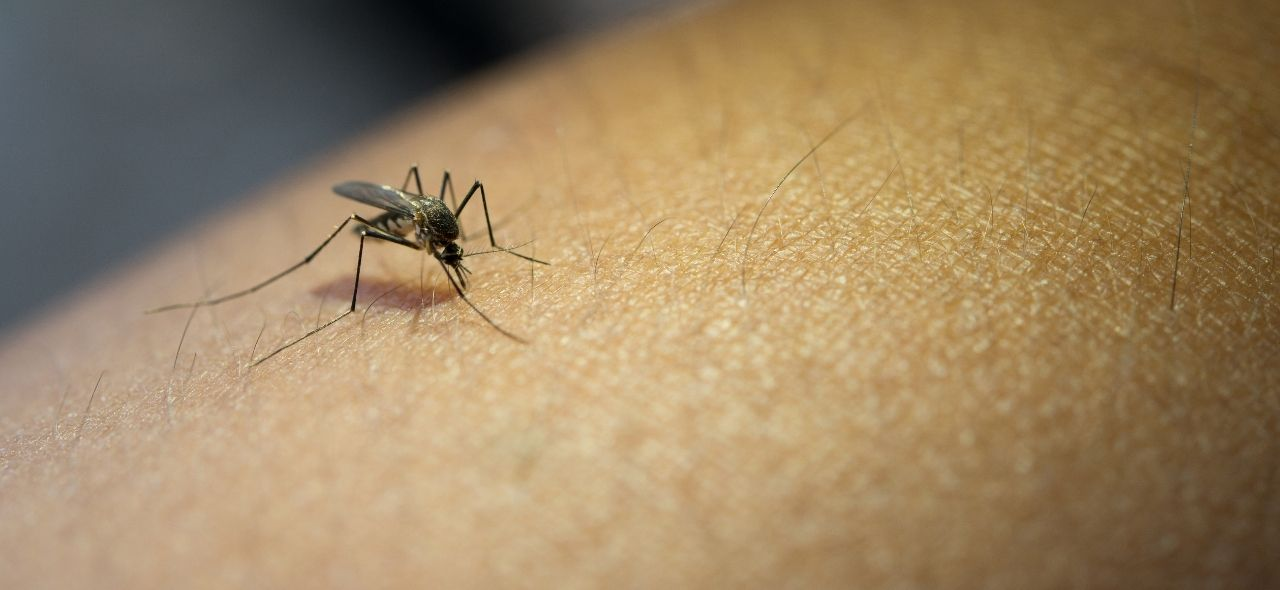
\includegraphics[width=0.8\textwidth]{figuras/Mosquito da Dengue.jpg}
	\label{fig:aedes_aegypti}
	\fonte{Ministério da Saúde, 2022.}
\end{figure}

A Figura~\ref{fig:aedes_aegypti} apresenta o mosquito \textit{Aedes aegypti}, facilmente identificável por suas listras brancas características nas pernas e uma marca em forma de lira no tórax, características morfológicas que auxiliam na identificação visual durante ações de vigilância entomológica.

A infecção por um sorotipo confere imunidade permanente e específica apenas para aquele sorotipo particular, havendo a possibilidade de infecções subsequentes pelos demais sorotipos. Essa característica imunológica aumenta o risco de desenvolvimento de formas graves da doença em infecções secundárias. A teoria aceita, conhecida como "hipótese de potência dependente de anticorpos" (Antibody-Dependent Enhancement - ADE), postula que anticorpos gerados em uma primeira infecção podem, paradoxalmente, facilitar a entrada do vírus heterotípico nas células do sistema imune (monócitos e macrófagos) durante uma segunda infecção, aumentando a carga viral e desencadeando uma resposta imune exacerbada. Essa resposta imune hiperativa pode levar a complicações graves, como extravasamento plasmático maciço, hemorragias espontâneas e choque hipovolêmico, características da Dengue Grave (anteriormente denominada Dengue Hemorrágica), que pode evoluir para a síndrome do choque da dengue e óbito caso não seja tratada adequadamente e em tempo hábil.

\subsubsection{Gravidade da doença e limitações impostas aos pacientes}

Os pacientes com dengue enfrentam limitações físicas, funcionais e sociais durante o período da doença. A fase febril inicial, que dura tipicamente de 3 a 7 dias, caracteriza-se por sintomas súbitos e intensos que aparecem abruptamente após o período de incubação intrínseca (4 a 10 dias após a picada do mosquito infectado). A febre alta súbita ($38-40~^\circ\mathrm{C}$), muitas vezes bifásica (com dois picos de temperatura), é acompanhada de dores musculares intensas e generalizadas que os pacientes frequentemente descrevem como "dor nos ossos", cefaleia severa e persistente, e dor retroorbital (atrás dos olhos) que piora com movimentos oculares. Esses sintomas comprometem a capacidade de realizar atividades cotidianas básicas, como trabalhar, estudar ou mesmo realizar tarefas domésticas simples.

Em casos graves, que ocorrem em aproximadamente 5-10\% das infecções e são mais comuns em infecções secundárias, os pacientes podem apresentar manifestações clínicas críticas. A magnitude do problema pode ser observada nos dados nacionais de incidência e óbitos por dengue, ilustrados na Figura~\ref{fig:dengue_incidencia_obitos}, que evidenciam a severidade crescente das epidemias no Brasil.

\begin{figure}[htb]
	\centering
	\caption{Incidência e óbitos por dengue no Brasil (janeiro de 2025)}
	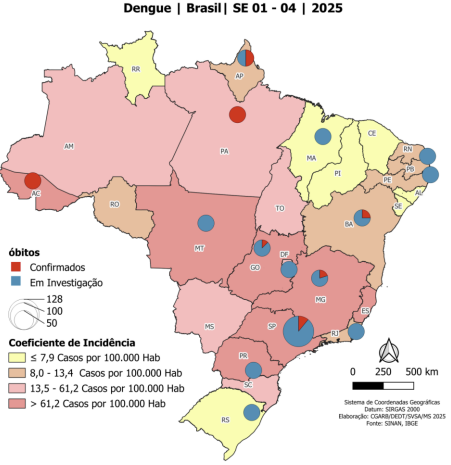
\includegraphics[width=0.6\textwidth]{figuras/Dengue Incidencia e Obitos Jan 2025.png}
	\label{fig:dengue_incidencia_obitos}
	\fonte{SINAN, IBGE, 2025.}
\end{figure}

As manifestações clínicas críticas incluem:

\begin{itemize}
    \item \textbf{Extravasamento de plasma:} O mecanismo fisiopatológico central da dengue grave é o aumento da permeabilidade vascular, resultando em extravasamento de plasma para os espaços extravasculares. Clinicamente, isso se manifesta como derrame pleural (acúmulo de líquido na cavidade torácica), ascite (acúmulo de líquido no abdome), derrame pericárdico e edema generalizado. Em casos severos, a perda de volume plasmático pode ultrapassar 20\% do volume sanguíneo total, levando a hipotensão arterial, taquicardia compensatória e, em última instância, choque hipovolêmico, exigindo hospitalização imediata em unidade de terapia intensiva, reposição volêmica agressiva com soluções cristaloides ou coloides, e monitoramento hemodinâmico contínuo.
    
    \item \textbf{Hemorragias:} A trombocitopenia (diminuição do número de plaquetas) e as alterações na função plaquetária, combinadas com distúrbios da coagulação, podem resultar em sangramentos espontâneos ou após procedimentos médicos (venopunção, injeções intramusculares). As manifestações hemorrágicas variam desde petéquias cutâneas e epistaxe (sangramento nasal) até hemorragia gastrointestinal, sangramento uterino anormal e, em casos extremos, hemorragia intracraniana, que pode ser fatal se não diagnosticada e tratada prontamente. Pacientes com sangramentos ativos podem necessitar de transfusão de plaquetas e plasma fresco congelado.
    
    \item \textbf{Comprometimento de órgãos:} A dengue pode causar disfunção orgânica múltipla. Hepatite por dengue, caracterizada por elevação de transaminases e icterícia, pode levar a insuficiência hepática aguda. A encefalite por dengue, resultante da invasão viral do sistema nervoso central ou de complicações da síndrome de choque, pode causar convulsões, alteração do nível de consciência e déficits neurológicos permanentes. Miocardite e insuficiência cardíaca aguda têm sido relatadas, especialmente em crianças. Insuficiência renal aguda pode ocorrer secundária ao choque ou diretamente por nefrotoxicidade viral, exigindo terapia dialítica temporária em casos severos.
\end{itemize}

Além das manifestações clínicas agudas, muitos pacientes desenvolvem sequelas de longo prazo que podem persistir por semanas ou meses após a resolução da fase aguda da infecção. A síndrome pós-dengue, ainda pouco estudada mas frequentemente relatada por pacientes e profissionais de saúde, caracteriza-se por fadiga crônica incapacitante, dores articulares e musculares persistentes, dificuldades de concentração e memória (popularmente conhecida como "neblina mental"), e depressão secundária. Estudos longitudinais sugerem que até 40\% dos pacientes que tiveram dengue grave podem apresentar sintomas persistentes após 3 meses da infecção aguda, impactando a qualidade de vida e a capacidade de retorno às atividades profissionais e acadêmicas.

\subsubsection{Perigos e impacto social}

O impacto da dengue transcende a esfera clínica individual, gerando um fardo multidimensional para a sociedade, a economia e o sistema de saúde. Epidemias de grande magnitude, como a observada no Distrito Federal em 2024, provocam uma cascata de efeitos deletérios que se propagam através de múltiplas camadas sociais e econômicas.

\paragraph{Ocupação e sobrecarga hospitalar}

A sobrecarga do Sistema Único de Saúde (SUS) é um dos impactos visíveis e imediatos. Durante picos epidêmicos, as unidades de atenção primária, pronto-atendimento e emergências hospitalares são inundadas com pacientes procurando atendimento, muitas vezes com sintomas leves ou moderados que poderiam ser manejados ambulatorialmente, mas que geram ansiedade e procura por serviços de saúde devido ao medo de complicações. Isso resulta em tempos de espera que podem ultrapassar 8-12 horas, comprometendo a qualidade do atendimento e aumentando o risco de erros médicos por sobrecarga dos profissionais. Leitos hospitalares, especialmente em unidades de terapia intensiva pediátrica e adulta, são rapidamente ocupados por pacientes com dengue grave, reduzindo a disponibilidade para outras emergências médicas, incluindo acidentes vasculares cerebrais, infartos do miocárdio e traumas. Durante a epidemia de 2024 no Distrito Federal, unidades de saúde relataram ocupação de leitos clínicos acima de 95\%, com pacientes sendo acomodados em corredores e espaços improvisados.

\paragraph{Mortalidade e impacto em vidas humanas}

Embora a maioria dos casos de dengue seja benigna, a mortalidade associada à doença representa um fardo humano imensurável. Óbitos por dengue ocorrem principalmente em casos graves que evoluem para síndrome do choque da dengue ou hemorragia grave, frequentemente associados a diagnóstico tardio ou acesso inadequado a cuidados de saúde. Durante a epidemia de 2024 no Distrito Federal, foram registrados dezenas de óbitos confirmados por dengue, muitos deles potencialmente evitáveis com diagnóstico precoce e tratamento adequado. Crianças, idosos e pessoas com comorbidades (diabetes, hipertensão arterial, doenças cardiovasculares) apresentam maior risco de evolução para formas graves e óbito. Além dos óbitos diretos, a dengue pode precipitar complicações em pacientes com condições preexistentes, contribuindo indiretamente para o aumento da mortalidade geral durante períodos epidêmicos.

\paragraph{Absenteísmo escolar e laboral}

O absenteísmo escolar e laboral durante epidemias atinge níveis críticos. Estudos econômicos estimam que, durante a epidemia de 2024 no DF, milhares de dias letivos foram perdidos por estudantes que estiveram doentes ou cuidando de familiares doentes. Escolas públicas e privadas reportaram ausências massivas de alunos e professores durante os picos da epidemia, comprometendo o calendário letivo e a qualidade do ensino. No ambiente de trabalho, a perda de produtividade é significativa: funcionários doentes ficam afastados por períodos que variam de 5 a 15 dias, dependendo da gravidade, enquanto outros podem precisar se ausentar para cuidar de filhos ou parentes doentes. Em setores essenciais, como educação, segurança pública e saúde, essas ausências podem comprometer o funcionamento básico dos serviços. O setor de serviços, incluindo comércio e turismo, também sofre impactos significativos durante epidemias, com redução no fluxo de clientes e turistas em áreas afetadas.

\paragraph{Custos econômicos diretos e indiretos}

Os custos econômicos diretos e indiretos são elevados. Estudos de análise de custo-efetividade estimam que o custo médio por caso de dengue no Brasil varia de R\$ 500 a R\$ 2.000, dependendo da complexidade do caso e da necessidade de hospitalização. Multiplicando esses valores pelos milhões de casos anuais, chega-se a um impacto econômico que pode ultrapassar R\$ 5 bilhões anualmente. Os custos diretos incluem gastos com consultas médicas, exames laboratoriais (sorologias, hemogramas, exames de função hepática e renal), medicamentos (analgésicos, antitérmicos, soluções de reidratação), internações hospitalares (incluindo custos de leitos de enfermaria e UTI), procedimentos diagnósticos e terapêuticos (transfusões de sangue e derivados, diálise em casos graves), e custos operacionais do sistema de saúde (sobrecarga de profissionais, horas extras, contratação temporária). Os custos indiretos, frequentemente subestimados, incluem perda de produtividade da força de trabalho, custos previdenciários por afastamentos (auxílio-doença, benefício previdenciário), impacto no turismo (áreas afetadas podem ter redução de visitantes e cancelamento de eventos), redução na arrecadação de impostos devido à queda na atividade econômica, e custos de oportunidade (recursos que poderiam ser investidos em outras áreas da saúde pública ou desenvolvimento social).

\paragraph{Desigualdades sociais e vulnerabilidade}

Populações vulneráveis, especialmente aquelas em áreas urbanas periféricas com infraestrutura sanitária precária, são desproporcionalmente afetadas, exacerbando desigualdades sociais existentes. Nessas comunidades, fatores como falta de abastecimento regular de água (levando ao armazenamento doméstico em recipientes que se tornam criadouros), coleta irregular de lixo (que acumula materiais que retêm água da chuva), e habitação precária (com telhados que permitem entrada de água) criam condições ideais para a proliferação do vetor. Além disso, o acesso limitado a serviços de saúde de qualidade, especialmente em horários de crise, significa que casos graves podem não receber atenção adequada em tempo hábil, aumentando o risco de complicações e óbitos evitáveis. Durante a epidemia de 2024 no Distrito Federal, dados mostraram que regiões administrativas com menor Índice de Desenvolvimento Humano (IDH) apresentaram taxas de incidência e letalidade por dengue superiores às áreas mais desenvolvidas, evidenciando a dimensão social e de equidade do problema.

\subsection{O que é Aprendizado de Máquina?}

Para profissionais de saúde pública, epidemiologistas e gestores que não possuem formação técnica em ciência da computação ou estatística avançada, é fundamental compreender de forma clara e didática o que são os métodos de aprendizado de máquina (\textit{Machine Learning}) e como eles podem ser aplicados para melhorar a vigilância epidemiológica da dengue. Esta subseção busca fornecer uma explicação acessível desses conceitos, utilizando analogias que facilitem a compreensão por parte de leitores com formação em áreas biológicas e médicas.

O aprendizado de máquina pode ser compreendido como uma abordagem computacional que permite que sistemas automatizados identifiquem padrões complexos em grandes volumes de dados históricos, aprendendo com exemplos passados para fazer previsões sobre eventos futuros. De forma análoga ao processo de aprendizado humano através da experiência, algoritmos de aprendizado de máquina são "treinados" utilizando dados históricos conhecidos (por exemplo, casos de dengue e variáveis climáticas dos últimos anos em todas as regiões do país), identificando relações e padrões que não seriam facilmente perceptíveis através de análise manual ou métodos estatísticos tradicionais. Após esse treinamento, o sistema é capaz de aplicar o conhecimento adquirido para fazer previsões sobre cenários novos e não observados anteriormente.

Para ilustrar esse conceito com uma analogia familiar ao contexto médico, imagine um médico experiente que, após anos de prática clínica atendendo pacientes com dengue, desenvolve uma capacidade intuitiva de reconhecer padrões sutis que indicam maior risco de complicações graves: combinações específicas de sintomas, histórico epidemiológico, características demográficas e fatores ambientais que, quando presentes simultaneamente, sugerem necessidade de monitoramento mais intensivo. O aprendizado de máquina opera de forma similar, mas de maneira sistemática e quantitativa: analisa milhares ou milhões de casos históricos, identifica quais combinações de variáveis (temperatura, precipitação, umidade, casos anteriores) estão associadas a surtos epidêmicos, e utiliza esse conhecimento para alertar sobre riscos futuros antes que os casos clínicos comecem a aparecer nos sistemas de notificação.

Uma característica fundamental que diferencia o aprendizado de máquina de métodos estatísticos tradicionais é sua capacidade de capturar relações não-lineares e interações complexas entre múltiplas variáveis simultaneamente. Enquanto análises estatísticas clássicas frequentemente assumem relações lineares (por exemplo, "um aumento de 1°C na temperatura resulta em um aumento proporcional de X casos de dengue"), o aprendizado de máquina pode identificar padrões mais sofisticados, como: "quando a temperatura está entre 24°C e 28°C E a precipitação acumulada nas últimas 4 semanas excede 150mm E a umidade relativa está acima de 70\%, então há alta probabilidade de um surto ocorrer nas próximas 6-8 semanas, mas esse padrão não se aplica se a temperatura anterior foi muito baixa". Essas relações complexas são particularmente relevantes para a dengue, uma vez que a dinâmica de transmissão envolve múltiplos fatores biológicos interconectados: o ciclo de vida do mosquito, o período de incubação viral, a disponibilidade de criadouros, e a suscetibilidade da população humana.

No contexto específico deste trabalho, o algoritmo adotado foi o XGBoost, que pode ser comparado a um sistema de decisão em árvore múltipla: o algoritmo constrói uma série de ``regras de decisão'' hierárquicas (semelhantes a fluxogramas clínicos) que avaliam diferentes combinações de variáveis climáticas e epidemiológicas para determinar o número esperado de casos. Cada ``árvore'' aprende a corrigir os erros das anteriores, resultando em um sistema de previsão progressivamente mais preciso. Tão importante quanto o modelo, porém, é a referência contra a qual ele é comparado: previsões de dengue apresentam forte dependência do passado recente, e uma regra trivial como ``a próxima contagem será igual à atual'' (a persistência) já acerta boa parte da dinâmica. Por isso, todos os modelos deste trabalho foram avaliados lado a lado com previsores ingênuos desse tipo, de forma que o ganho atribuído ao aprendizado de máquina seja medido, e não presumido.

É importante destacar que o aprendizado de máquina não substitui o conhecimento especializado de profissionais de saúde ou epidemiologistas, mas sim amplifica e sistematiza a capacidade de análise, permitindo processar volumes de dados que seriam impraticáveis para análise manual. Da mesma forma que exames laboratoriais e de imagem complementam o diagnóstico clínico sem substituir o julgamento médico, modelos preditivos baseados em aprendizado de máquina fornecem informações quantitativas adicionais que podem fundamentar decisões de saúde pública, como alocação de recursos, intensificação de controle vetorial, e preparação de unidades de saúde para períodos de alta demanda. A transparência e interpretabilidade dos modelos desenvolvidos neste trabalho são aspectos prioritários, garantindo que os resultados possam ser compreendidos e validados por profissionais de saúde pública, e não funcionem como "caixas-pretas" inacessíveis.

\subsection{Do TCC 1 ao TCC 2: evolução do escopo}

A primeira etapa deste trabalho (TCC~1) concentrou-se no Distrito Federal, utilizando a estação meteorológica de Brasília (A001) e a série de casos do DF, e propôs a comparação entre um modelo estatístico clássico (SARIMA) e um modelo de aprendizado de máquina (XGBoost). A análise exploratória daquela etapa indicou que um único município, com poucas centenas de semanas de observação e um único ano epidêmico extremo, oferece pouca informação para treinar e, sobretudo, para avaliar de forma confiável um modelo preditivo: o evento de 2024 no DF seria, ao mesmo tempo, o caso mais importante e o menos representado nos dados.

Por esse motivo, o TCC~2 ampliou o escopo para todo o território nacional. Os microdados do SINAN foram processados para os 5.570 municípios brasileiros, as cerca de 700 estações automáticas do INMET foram associadas geograficamente a esses municípios, e a série foi agregada no nível das 137 mesorregiões geográficas definidas pelo IBGE \cite{ibge1990mesorregioes}. Essa escala intermediária preserva a heterogeneidade regional descrita na literatura e, ao mesmo tempo, reduz o ruído das contagens municipais pequenas e a dependência de uma única estação meteorológica. O Distrito Federal, que corresponde a uma mesorregião, permanece como recorte de análise nos resultados.

Durante a execução, a auditoria dos dados revelou defeitos que invalidavam versões anteriores da análise, entre eles um deslocamento no mapeamento das colunas dos arquivos do INMET que fazia a variável tratada como ``umidade relativa'' corresponder, na verdade, à temperatura do ponto de orvalho. A correção desses defeitos, e a medição de quanto cada um alterava os resultados, tornou-se parte da contribuição metodológica do trabalho, descrita no Capítulo~\ref{cap:metodologia}.

\section{Pergunta de Pesquisa}

Considerando o cenário epidemiológico nacional, o potencial das variáveis climáticas como preditores antecipados e a necessidade de transicionar de uma vigilância reativa para uma vigilância preditiva baseada em evidências quantitativas, este trabalho propõe-se a responder à seguinte questão central:

\begin{quote}
\textit{Em que medida um modelo de aprendizado de máquina (XGBoost), treinado com a série histórica de notificações de dengue do SINAN e com variáveis climáticas do INMET defasadas segundo o ciclo biológico do vetor, é capaz de prever o número de notificações de dengue com quatro semanas de antecedência nas mesorregiões brasileiras, quanto as variáveis climáticas acrescentam a essa previsão e como o modelo se compara a previsores ingênuos, inclusive em um evento epidêmico extremo como o de 2024?}
\end{quote}

A pergunta desdobra-se em três questões operacionais, respondidas no Capítulo~\ref{cap:resultados}: (i) qual o desempenho do modelo frente a baselines ingênuos (persistência, média móvel e sazonalidade); (ii) qual o ganho, estatisticamente testado, da inclusão das variáveis climáticas, inclusive em cenários em que os dados epidemiológicos recentes não estão disponíveis; e (iii) quais variáveis e limiares climáticos o modelo efetivamente utiliza.

\section{Objetivos}

\subsection{Objetivo Geral}

Desenvolver e avaliar um modelo de previsão semanal de notificações de dengue para as 137 mesorregiões brasileiras, com horizonte de quatro semanas, baseado em XGBoost e em dados integrados do SINAN e do INMET, quantificando rigorosamente a contribuição das variáveis climáticas e comparando o modelo a previsores ingênuos, e disponibilizar os resultados por meio de uma API e de um painel de visualização.

\subsection{Objetivos Específicos}

\begin{enumerate}
    \item \textbf{Construir um pipeline reprodutível de dados:} processar os microdados nacionais do SINAN (OpenDataSUS) e os dados horários das estações automáticas do INMET em camadas Bronze, Silver e Gold, agregando-os por semana epidemiológica e mesorregião, com verificações automáticas de qualidade e integridade.

    \item \textbf{Auditar e corrigir a qualidade dos dados:} identificar e corrigir defeitos de extração e agregação (mapeamento de colunas, valores zero indevidos, semanas partidas na virada do ano, lacunas de anos inteiros) e medir o efeito de cada correção sobre os resultados.

    \item \textbf{Construir atributos com base no ciclo biológico do vetor:} gerar defasagens de 1 a 8 semanas, médias móveis nas janelas de 2 a 4 e de 4 a 8 semanas e anomalias climáticas calculadas exclusivamente sobre o período de treino.

    \item \textbf{Treinar e comparar modelos com e sem clima:} treinar três variantes do XGBoost (apenas dados epidemiológicos; com clima bruto; com clima enriquecido) e compará-las entre si e com três baselines ingênuos, sob um protocolo de validação temporal que impeça o vazamento de informação do futuro.

    \item \textbf{Avaliar a robustez e a utilidade do clima:} testar o desempenho ano a ano, por meio de validação \textit{walk-forward}, em simulações de atraso na notificação (\textit{data blindness}) e no evento epidêmico de 2024, e interpretar o modelo por meio de valores SHAP.

    \item \textbf{Disponibilizar os resultados:} expor as previsões e os alertas em uma API REST e em um painel interativo de visualização.
\end{enumerate}

\section{Contribuições}

As principais contribuições deste trabalho são:

\begin{itemize}
    \item um pipeline nacional, reprodutível e versionado de integração SINAN--INMET em nível de mesorregião, com verificações que abortam a execução diante de inconsistências na série;
    \item a documentação de defeitos de dados que afetam análises baseadas nos arquivos públicos do INMET e do SINAN, com a medição do seu efeito, incluindo a constatação de que uma associação entre ``umidade'' e dengue observada em versões preliminares era um artefato de mapeamento;
    \item uma avaliação do XGBoost que o compara com baselines ingênuos, e não apenas com variações de si mesmo, e que separa o desempenho em anos típicos do desempenho no evento extremo de 2024;
    \item a quantificação do ganho das variáveis climáticas, pequeno mas estatisticamente consistente, e de seu papel quando os dados epidemiológicos recentes estão ausentes.
\end{itemize}

\section{Organização do Trabalho}

O Capítulo~\ref{cap:referencial} apresenta a fundamentação teórica sobre a dengue, sua relação com o clima e os métodos de previsão e de interpretação utilizados. O Capítulo~\ref{cap:metodologia} descreve as bases de dados, o pipeline, as correções de qualidade, a engenharia de atributos e o protocolo experimental. O Capítulo~\ref{cap:resultados} apresenta e discute os resultados. O Capítulo~\ref{cap:sistema} descreve a API e os painéis desenvolvidos. O Capítulo~\ref{cap:conclusao} reúne as conclusões, as limitações e os trabalhos futuros, e o Capítulo~\ref{cap:cronograma} registra o cronograma executado.
